\section*{Общая характеристика работы}
%\fontsize{14pt}{15pt}\selectfont
% paragraph - меньше шрифт
% зеленые гиперссылки

\paragraph{Актуальность темы исследования.} К подземным грызунам относят примерно 250 видов, проводящих всю или почти всю свою жизнь под землей. Они распространены по всем континентам за исключением Австралии и Антарктиды (\cite{Fang2015}). Уход под землю помогает избежать открытых контактов с хищниками и сильных температурных колебаний, но приводит к возникновению новых стрессовых факторов: темнота, кислородная недостаточность и гиперкапния, повышенный инфекционный фон. Существование в этих условиях приводит к формированию сходных морфо-физиологических адаптаций у филогенетически далеких форм. Несмотря на изученность морфологических адаптаций, молекулярные основы этого процесса остаются не до конца понятными. К настоящему моменту в открытых базах данных уже накопилось достаточное количество последовательностей как отдельных генов, так и полногеномных данных, позволяющих проводить сравнения на различных таксономических уровнях.

Подсемейство полевочьи (Arvicolinae) -- одна из самых молодых и многочисленных групп отряда, распространенная практически во всех ландшафтных зонах Северного полушария. Они представляет собой удобную модель для тестирования гипотез о темпах и формах адаптивной эволюции, прежде всего связанную с роющим и подземным образом жизни. Предыдущие исследования молекулярных адаптаций к подземному образу жизни выполнялись на немногочисленных и полностью подземных представителях филогенетически далеких таксонов из разных семейств и подотрядов (слепыши, землекопы, туко-туко). Полевки, в свою очередь, предоставляют уникальные возможности для тестирования гипотез об универсальности этих механизмов за счет сравненения близкородственных пар подземных и наземных видов в пределах одного семейства. 


% морфо-фзиологическе адаптации изучались. Значительно меньше мы знаем о молекулярных механизмах, которые изучались сильно хуже. 

%Подземные грызуны являются прекрасным модельным объектом эволюционной биологии для изучения адаптаций к подземному образу жизни. Более того, сравнение их с родственными наземными видами с использованием молекулярных подходов может способствовать выявлению процессов формирования адаптаций, начиная с молекулярного уровня. 

%рассказ о подсемействе, его преимущества (морфологически изучалось, молекулярно очень плохо, можем изучить начальные стадии адаптациии есть градации адаптации к подземному образу жизни) и том, как изучалось на других видах и в чем были проблемы


\paragraph{Степень разработанности темы исследования.} Несмотря на очень интенсивную историю исследования подсемейства с применением молекулярных методов, мало что известно относительно молекулярных механизмов их быстрой адаптивной радиации. За относительно недолгий период эволюции группы ее представители независимо переходили к жизни под землей. Предыдущие исследования молекулярных адаптаций к подземному образу жизни выполнялись на немногочисленных и полностью подземных представителях филогенетически далеких таксонов из разных семейств и подотрядов (слепыши, землекопы, туко-туко). 

%До настоящий исследований изучение молекулярных механизмов на подсемействе не проводилось

Среди подземных полевочьих активно изучались только молекулярные адаптации \textit{Lasiopodomys mandarinus}. Однако, авторы исследований проводили сравнения не в рамках подсемейства, а с отдельными подземными грызунами из других филогенетически очень далеких семейств (\textit{Heterocephalus glaber}, \textit{Fukomys damarensis} и несколькими видами рода \textit{Spalax}) (\cite{Sun2020};\cite{Sun2018a}; \cite{Dong2020}).

Не смотря на то, что в подсемействе есть другие виды, которые независимо перешли к подземному образу жизни, исследования их молекулярных адаптаций не проводилось. Также как и не делались сравнения и анализ конвергенции молекулярных признаков с другими более эволюционно древними подземными грызунами.

\paragraph{Цели и задачи работы.} Целью данной работы является проведение молекулярно-генетических сравнениий филогенетически независимых подземных форм подсемейства полевочьих (Arvicolinae, Cricetidae, Rodentia) и их наземных сестринских таксонов и выявление следов отбора при освоении подземной ниши на молекулярном уровне.
%\vspace{0pt plus0.5fill}

Для достижения поставленной цели были сформированы следующие задачи:
\begin{enumerate}
	\item Сравнить направление и силу отбора для гена \textit{CYTB}, митохондриальных и ядерных белок-кодирующих генов у подземных и наземных грызунов;
	\item Провести поиск параллельных аминокислотных замен в ядерных и митохондриальных генах в независимых линиях подземных полевочьих;
	\item Выявить функции генов с измененным увронем отбора относительно наземных грызунов и параллельными аминокислотными заменами, определить биохимические процессы, в которые они вовлечены;
	\item Сравнить количество генов со следами адаптации к подземному образу жизни, среди подземных представителей подсемейства Arvicolinae;
	\item Провести сравнение геномных изменений у эволюционно молодых подземных полевочьих с представителями эволюционно более древних семейств подземных грызунов. 
\end{enumerate}

\paragraph{Научная новизна.} В рамках работы впервые проведены масштабные исследования представителей подсемества полевочьи (Arvicolinae, Rodentia) для поиска следов конвергентной эволюции в филогенетически независимых линиях подземных грызунов. Исследование проведено в разном масштабе: от анализа отдельного филогенетического маркера \textit{CYTB} до пула ядерных белок-кодирующих генов. Впервые проанализированы паттерны аминокислотных замен и выявлены сайты с параллельными заменами. Для всех белок-кодирующих митохондриаьлных и ряда ядерных (112) генов была проведена оценка силы и направления отбора несколькими методами (codeml branch model, RELAX, aBSREL). В ходе выполнения работы в лаборатории эволюционной геномики и палеогеномики ЗИН РАН было получено 36 новых митохондриальных геномов и более 15 транскриптомов, что представляет существенный вклад для дальнейшего изучения эволюционной истории подсемейства. 

\paragraph{Теоретическая и практическая значимость работы.} В работе получены фундаментальные данные, описывающие молекулярные адпатции к подземному образу жизни представителей подсемейства полевочьи. Также впервые дана сравнительная характеристика различий в уровне отбора между филогенетически независимыми подземными видами. Обнаруженные гены с измененным уровнем отбора и параллельными заменами могут служить источником для более детального изучения адаптивной и эволюционной физиологии. Собранные и опубликованные в открытом доступе митохондриальные геномы и транскриптомы будут использованы в работах по филогеографии, филогении и изучении других эволюционных процессов внутри подсемейства Arvicolinae сотрудниками как Зоологического института РАН, так и учебных и научных заведений всего мира. Результаты исследования могут быть использованы в курсах лекций по эволюционной биологии в вузах, школах и секциях дополнительного образования.

\paragraph{Положения, выносимые на защиту.}
\begin{enumerate}
	\item Наблюдается ослабление уровня отбора в большинстве митохондриальных белок-кодирующих генах у подземных форм полевочьих. 
	\item У подземных форм подсемейства полевочьи присутствуют параллельные аминокислотные замены в генах, которые вовлечены в процессы адаптации к низкой концентрации кислорода.
	\item Интенсивность уровня отбора на митохондриальные и ядерные гены коррелирует с со степенью специализации к подземному образу жизни и не зависит от возраста таксона.
	\item Направления адаптивной изменчивости у подземных форм полевочьих имеют тот же характер, что и в других древних специализированных подземных грызунов семейств Spalacidae, Ctenomyidae, Bathergidae.
\end{enumerate}

\paragraph{Степень достоверности и апробации результатов.} Материалы диссертации были представлены на 7 международных конверенциях и конгрессах: международных конференцииях по вычислительной биологии MCCMB в 2017 и 2019 г. (Москва, Россия); XI международной конференции по биоинформатике и системной биологии BGRS (Новосибирск, 2018); 16 международной конференции Rodens et Spatium (Потсдам, Германия, 2018); VII международном конгрессе общества генетиков и селекционеров ВОГиС (Санкт-Петербург, 2019); 45 конгрессе федерации европейского биохимического сообщества (FEBS) (дистанционно, 2021); XI Съезде Териологического общества при РАН (2022). Материалы также были представлены на итоговой отчетной сессии ЗИН РАН в 2020 году, семинарах лаборатории эволюционной геномики факультета биоинформатики и биоинженерии МГУ (Москва, 2018, 2021) и биоинформатическом семинаре Университета ИТМО (2022).

\paragraph{Публикации.} Основные результаты по теме диссертации изложены в 15 печатных изданиях, из них 7 статей в журналах, рекомендованных ВАК и 8 --- тезисы научных докладов.

\paragraph{Объем и структура работы.} Работа состоит из введения, трех глав, заключения, выводов и списка литературы. Основная часть работы изложена на 75 страницах, содержит 15 рисуноков и 12 таблиц. Список литературы включает 147 наименований, из которых 7 на русском языке и 140 -- на английском. Приложения к работе содержит 4 таблицы на 16 страницах.

%\underline{\textbf{Благодарности}}
\paragraph{Благодарности.}
%\begin{small}
В первую очередь хочу поблагодарить мою научную руководительницу Наталью Иосифовну Абрамсон за помощь и поддержку при выполнении диссертации, ценные советы и доверие в выборе методик анализа. Отдельную благодарность хотелось бы выразить всему коллективу лаборатории эволюционной геномики и палеогеномики ЗИН РАН за неоценимый вклад в мое зоологическое образование, освоение филогенетических и филогеографических методик: Семену Бодрову, Татьяне Петровой и Евгению Генельт-Яновскому. За помощь в изучении биоинформатических подходов искренне благодарю Институт биоинформатики, а за обсуждение полученных результатов и ценные замечания -- А.В. Сморкачеву и сотрудников ИППИ РАН, ФББ МГУ и ИОГеН РАН: Надежду Потапову, Артема Касьянова, Алексея Пенина, Марию Логачеву, Егора Базыкина и А.С. Кондрашова.   

За моральную поддержку во время написания работы хочу поблагодарить в первую очередь своего супруга Станислава Бондарева, а также Евгения Генельт-Яновского, Ольгу Бочкареву, Александру Пантелееву, Анну Гнетневу, Анну Ганюкову, членов моей семьи, друзей и коллектив Института биоинформатики. Отдельную благодарность хочу выразить моей бабушке, Паненковой Галине Ильиничне, которая до конца верила, что у меня все получится. 

За помощь в организации рабочего времени выражаю огромную благодарность Татьяне Смирновой и Екатерине Копейкиной, без которых получение результатов и написание диссертации заняло бы гораздо больше времени. Отдельную благодарность выражаю композиторам компаний CR Project Red, Guerrilla Games и FromSoftware, под произведения которых данная работа была написана. 

Работа выполнена в рамках темы государственного задания № AAAA–A19–119020790106–0 в лаборатории эволюционной геномики и палеогеномики ЗИН РАН. Исследования поддержаны грантами РФФИ №18-04-00730, №15-04-04602, №18-34-20118 и РНФ № 19-74-20110.

%\end{small}

\newpage
\section*{Содержание работы}

\subsection*{Глава 1. Обзор литературы.}
Глава представлена тремя разделами. Первый раздел посвящем описанию морфо-физиологических изменений у грызунов, которые возникают при переходе к подземному образу жизни. Второй раздел освещает изучение молекулярных адаптаций подземных грызунов и показывает потенциальную возможность адаптивных изменений генов как в митохондриальном, так и в ядерном геномах. Третий раздел посвящен подсемейству Arvicolinae, описанию основных подземных представителей этого подсемейства и обзору изучения молекулярных адаптаций у его представителей. 


\subsection*{Глава 2. Материал и методы}

Работа включает в себя поиск следов отбора в разном масштабе: в пределах одного митохондриального филогенетического маркера \textit{CYTB}, среди полных митохондриальных геномах и ядерных генах. Количество видов, взятых в анализ на каждом из этапов, отличается из-за доступности материала и количества данных, выложенных в открытый доступ в базе данных GenBank. Ген \textit{CYTB} был выбран как самый распространенный филогенетический маркер и, следовательно, дал возможность взять в анализ большое количество подземных и наземных видов. В каждом случае мы использовали максимально репрезентативную филогенетическую выборку из доступных на момент исследования видов для адекватного таксономического контекста.Все сиквенсы, проанализированные в рамках данной работы, были получены из материала коллекции или из открытой базы данных GenBank (https://www.ncbi.nlm.nih.gov/genbank/).

\textbf{Выделение ДНК.} Образцы мышечной и кожной ткани хранили в 96\% этаноле при -20 $^\circ$С в коллекции тканей и ДНК группы молекулярной систематики млекопитающих Зоологического института РАН.  

Для амплификации методом Сенгера геномную ДНК выделяли с использованием стандартного протокола солевой экстракции (\cite{Miller1999}). Выделение ДНК проводили в специально оборудованной лаборатории эволюционной геномики и палеогеномики ЗИН РАН (Английский проспект 32, Санкт-Петербург, Россия).

Для получения коротких ридов методом NGS (next generation sequencing) геномную ДНК экстрагировали с помощью Diatom DNA Prep 200 (Isogen, Россия). Ультразвуковая фрагментация проводилась с использованием сфокусированного ультразвукового прибора Covaris S220 (Covaris). Полученную фрагментированную ДНК очищали и концентрировали с использованием парамагнитной химии на основе гранул AMPure XP (Beckman-Coulter), применяя стандартные протоколы. Концентрацию оценивали флуориметром Qubit (Thermo Fisher). Выделение ДНК проводили в центре коллективного пользования в области геномики Сколтеха (https://www.skoltech.ru/research/en/shared-resources/gcf-2/).

\textbf{Выделение РНК}. Образцы смешанных тканей для получения транскриптомов хранили в фиксаторе intactRNA (Евроген, Россия) в коллекции тканей и ДНК лаборатории эволюционной геномики и палеогеномики ЗИН РАН. 

Выделение РНК из тканей производилось с использованием набора для выделения RNeasy mini kit (Qiagen) по протоколу для выделения из клеток животных (animal cells/spin) со следующими модификациями: 1) на шаге 4 добавляли 0.5 объема 96 \% EtOH; 2) после добавления спирта помещали пробирку в термостат на 37 $^\circ$С на 2 минуты, 3) элюция проводилась 30 мкл RNase-free water. Гомогенизацию проводили при помощи растирания пестиком в ступке в жидком азоте. Целостность РНК (RIN) определяли с помощью капиллярного электрофореза на приборе Bioanalyzer 2100 (Agilent). Для дальнейшей работы использовали образцы с RIN не менее 7. Выделение РНК проводили в центре коллективного пользования в области геномики Сколтеха (https://www.skoltech.ru/research/en/shared-resources/gcf-2/).


\textbf{Амплификация отдельных генов}. В первой части работы для лучшего разрешения филогенетического дерева Arvicolinae, необходимого для анализа изменчивости гена \textit{CYTB}, наряду с самим геном были использованы и семь ядерных: ген рака груди 1 (\textit{BRCA1}), экзон 11; ген рецептора гормона роста (\textit{GHR}), экзон 10; фрагмент гена лецитин-холестерин-ацилтрансферазы (\textit{LCAT}), экзоны 2-5 и интроны 2-4; ген белка-супрессора опухолей (\textit{PT53}), экзоны 5-7 и интроны 5-6; ген интерфоторецепторного ретиноид-связывающего белка (\textit{IRBP}); ген фактора фон Виллебранда (\textit{vWF}), экзон 28; и ген кислой фосфатазы типа V (\textit{Acp5}), экзоны 2 и 3. ПЦР-очистку проводили с использованием набора Omnix («Омникс», Россия). ПЦР-продукты секвенировали в обоих направлениях с использованием ABI BigDye версии 3.1. на автоматическом капиллярном секвенаторе Genetic Analyzer 3130 (Applied Biosystems) в компании Евроген (https://evrogen.ru/). 

\textbf{Получение ридов для сборки митохондриальных геномов}. Для подготовки библиотек ДНК для NGS секвенирования был использован набор NEBNext Ultra II DNA Library Prep Kit for Illumina (New England Biolabs). Приготовление библиотек производилось по протоколу со следующими изменениями: 1)  очистка на магнитных частицах после лигирования проводилась по пункту 3В (without size selection) в соотношении объем образца к объему магнитных частиц -- 1:0,9; 2) число циклов в ПЦР -- 10.
Полученные в результате ПЦР продукты были очищены и концентрированы при помощи магнитных частиц в соотношении объем образца к объему магнитных частиц -- 1:0,9. Элюция проводилась в 20 мкл бидистиллированной воды. Концентрация образцов измерялась на флуориметре Qubit.
Проверка качества полученных библиотек проводилась при помощи Bioanalyzer 2100 Agilent с помощью набора DNA High Sensitivity kit.

Секвенирование проводили на приборе HiSeq4000 (Illumina) со следующими параметрами: длина чтения 75, парные чтения. Качество отсеквенированной ДНК проверяли с помощью Qubit, окончательное распределение длин проверок содержимого адаптера библиотек проводили с помощью Bioanalyzer2100 (Agilent). Демультиплексирование и перевод данных в формат fastq проводили с помощью программы bcl2fastq2. Секвенирование проводили в центре коллективного пользования в области геномики Сколтеха (https://www.skoltech.ru/research/en/shared-resources/gcf-2/).

\textbf{Получение ридов для сборки транскриптомов}. Для выделения полиА-РНК из общей фракции РНК и дальнейшей подготовки ДНК-библиотек использовался совмещенный протокол набора NEBNext Poly(A) mRNA Magnetic Isolation Module и набора NEBNext Ultra II Directional RNA Library Prep Kit for Illumina (https://international.neb.com/protocols/). Подготовка проводилось по протоколу со следующими модификациями: 
1) фрагментация образцов проводилась на 94$^\circ$С 10 минут; 
2) синтез первой цепи проводился, используя программу со следующими параметрами: 25$^\circ$С -- 10 минут, 42$^\circ$С -- 30 минут, 70$^\circ$С -- 15 минут; 
3) очистка и концентрирование ДНК проводилось по протоколу при помощи магнитных частиц Ampure XP. Элюция проводилась бидистиллированной водой; 
4) число циклов в ПЦР -- 10 или 15, в зависимости от исходной концентрации РНК. 
Концентрация образцов измерялась на флуориметре Qubit. Проверка качества полученных библиотек проводилась при помощи Bioanalyzer 2100 Agilent с помощью набора DNA High Sensitivity kit. 

Секвенирование проводили на приборе HiSeq4000 (Illumina) со следующими параметрами: длина чтения 75, парные чтения. Демультиплексирование и перевод данных в формат fastq проводили с помощью программы bcl2fastq2. Секвенирование проводили в центре коллективного пользования в области геномики Сколтеха (https://www.skoltech.ru/research/en/shared-resources/gcf-2/).

\textbf{Сборка и аннотация митохондриальных геномов и транскриптомов}. Качество сырых чтений оценивалось с помощью FastQC (\cite{Andrews2010}). Очищение от адаптеров или фрагментов с низким качеством проводилось с помощью программы Trimmomatic (\cite{Bolger2014}). В работу брали риды только качеством выше 28-29.

Поскольку выделение митохондриальной ДНК \textit{Hyperacrius fertilis} производилось из коллекционных образцов прошлого века, это могло сказаться на качестве отсеквенированных последовательностостостей. Для оценки качества ридов дополнительно использовали программу mapDamage 2.0 (\cite{Jonsson2013}), отображающую паттерны неправильного включения нуклеотидов и процессов деазминирования. 

Сборка \textit{de novo} митохондриальных геномов осуществлялась программой plasmid SPAdes (\cite{Bankevich2012}) с настройками по умолчанию. Полученные контиги были отфильтрованы по длине. Для дальнейшей аннотации отобирали контиг с наибольшим сходством по размеру с митохондриальной ДНК для млекопитающих примерно 16 т.п.н. Контиги были аннотированы с помощью веб-сервера MITOS (\cite{Bernt2013}) с настройками по умолчанию и с учетом митохондриального генетического кода позвоночных. Границы генов были проверены и уточнены при сравнении с 21 опубликованной последовательностью митогенома Arvicolinae. Все позиции с низким качеством и покрытием, а также фрагменты, сильно отличающиеся от ранее опубликованных митохондриальных геномов Arvicolinae, были заменены на N вручную. Последовательности белок-кодирующих генов проверяли на содержание преждевременных стоп-кодонов вручную.

Tранскриптомы собирали стандартным пакетом Trinity (\cite{Grabherr2011}) с настройками по умолчанию. Поиск кодирующих участков собранных транскриптов проводили программой Transdecoder (https://github.com/TransDecoder/). Полученные последовательности очищали от химерных генов программой DIAMOND (\cite{Buchfink2015}), беря для сравнения нуклеотидную базу NCBI (nr). Ортологичные гены определяли с помощью Proteinortho (\cite{Lechner2011}). Полученные ортологи фильтровали в среде R 3.4.4 (\cite{RCoreTeam2017}), оставляя только те гены, которые встречаются в одной копии у всех взятых в анализ видов. 

\textbf{Оценка нуклеотидного состава митохондриальных геномов}. Базовый нуклеотидный состав (процентное содержание каждого из нуклеотидов) был рассчитан в Geneious Prime 2019.1 (https://www.geneious.com). Смещение в нуклеотидном составе (GC-skew) было оценено как $CG_{skew} = \frac{C - G}{C + G}$ (\cite{Arabi2010}; \cite{Hassanin2005}) с помощью пакета BioSeqUtils в BioPython (\cite{Cock2009}) в среде Python 3.0. 

\textbf{Выравнивание}. Последовательности гена \textit{CYTB}, ядерных генов и полных митохондриальных геномов были выровнены с помощью программы Mauve 1.1.1 (\cite{Darling2004}), реализованной как плагин Geneious Prime 2019.1 (https://www.geneious.com). Конкатенированная последовательность 13 белок-кодирующих митохондриальных генов была отдельно выровнена с использованием MAFFT 7.222 (\cite{Katoh2014}). Ядерные ортологичные гены по отдельности были выровнены программой prank (http://wasabiapp.org/software/prank/) с учетом триплетности кодирующей последовательности. Общие для всех фрагмены выравнивания редактировали вручную. Выравнивания конкатенировались в единую последовательность скриптом на языке программирования Python3.

\textbf{Филогенетическая реконструкция}. Для анализа изменчивости \textit{CYTB} было построено филогенетическое дерево на основе конкатенированных гена \textit{CYTB} и семи ядерных генов (\textit{BRCA1}, \textit{GHR}, \textit{LCAT},\textit{PT53}, \textit{IRBP}, \textit{vWF}, \textit{Acp5}). Наилучшее соответствие моделей замены для каждого гена оценивалось с помощью Treefinder (\cite{Jobb2004}) в соответствии с скорректированным информационным критерием Акаике (AICc). Байесовский анализ на основе конкатенированного выравнивания был проведен в MrBayes 3.2.6 (\cite{Ronquist2012}). Для оценки отбора на митоходриальные гены была создана филогенетическая реконструкция, включавшая 57 видов подсемейства полевочьих и 6 видов в качестве внешней группы. Реконструкция проводилась в программе MrBayes 3.2.2 (\cite{Ronquist2012}), используя 13 белок-кодирующих генов (11 417 п.н.). Были заданы следующие параметры анализа: nst=mixed и гамма-распределение скоростей замен между сайтами, использовалось деление на партиции по генам. 

Каждый анализ начинался со случайных деревьев, и два независимых прогона с 4 Марковскими цепями Монте-Карло (MCMC) выполнялись для 5 миллионов поколений, с выборкой каждого 1000-го поколения. Стандартные отклонения разделенных частот были ниже 0.01, потенциальные коэффициенты уменьшения масштаба были равны 1.0, а сходимость оценивали с помощью статистики ESS в Tracer v1.6 (\cite{Rambaut2014}). Консенсусное дерево было построено на основе деревьев, отобранных после 25\% отжига. Дерево визуализировали в программе FigTree v1.4 (http://tree.bio.ed.ac.uk/software/figtree/).

Конкатенированное выравнивание ядерных ортологичных генов было очищено от неинформативных сайтов программой Gblocks (\cite{Castresana2000}). Деревья были построены по полному и очищенному выравниванию с помощью программы RAxML (\cite{Stamatakis2014}) с конкатенированием методом Majority Rule с 500 репликами бутстрепа. 

\textbf{Оценка аминокислотных замен и их распределения}. Достоверные физико-химические аминокислотные изменения между остатками в \textit{CYTB} были обнаружены с использованием модифицированной модели MM01, реализованной в TreeSAAP v3.2 (\cite{Woolley2003}). Восемь категорий (1–8) использовались для представления величины радикальных замен, из которых категории от 6 до 8 указывают на наиболее радикальные замены (\cite{McClellan2001}). Значимые положительные значения (категории 6-8, P <0,001) были приняты как признак значимого изменения функции белка. 

Распределение синонимичных и несинонимичных замен было рассчитано между подземными и наземными видами на каждом участке гена \textit{CYTB} отдельно и объединены по координатам доменов. Значимость частоты замещения оценивалась с помощью точного критерия Фишера и поправки на множественное сравнение методом Холма. Все расчеты проводились в программе R v.3.4.4. Координаты доменов были получены на сайте UniProt по координатам \textit{CYTB} \textit{Mus musculus}: https://www.uniprot.org/uniprot/P00158. Частоты использования аминокислот для каждой позиции гена \textit{CYTB} определяли с использованием всех последовательностей для выбранных видов, чтобы учесть внутривидовые вариации. Этот набор данных включал все в базе данных Genbank по всем взятым в анализ видам на август 2020 года. Аминокислотные паттерны были рассчитаны с использованием скрипта на Python 3. Тест Фишера для сравнения частот считали с учетом неравных размеров выборки, поправку на множественное сравнение проводили методом Холма в статистической среде R.

Оценку замен в митохондриальных геномах и транскриптомах проводили программой ProtParCon (github.com/iBiology/ProtParCon) с дальнейшим поиском аминокислот, характерных только для подземных грызунов. Поиск осуществлялся с помощью рукописного скрипта на языке программирования Python 3. Оценку достоверности обнаруженных замен проводили с помощью функции ProtParCon с дальнейшей поправкой Холма на множественное сравнение вручную в в статистической среде R. 

\textbf{Оценка уровня и направления отбора}. Количество несинонимичных (\textit{dN}) и синонимичных (\textit{dS}) замен, а также $\omega$ (их соотношение) были рассчитаны несколькими способами. В каждом случае уровень и направление отбора были рассчитаны независимо для подземного вида (или рода) и его филогенетически близких наземных видов (рис. \ref{tree_mito}). 
\begin{itemize}
	\item[\textbullet] С использованием codeml, реализованного в ete-toolkit (\cite{Huerta-Cepas2016}). Для каждого подземного вида было проведено несколько анализов: с использованием модели со свободными ветвями (b\_free, где $\omega$frg и $\omega$bkg свободны), нейтральная модель (b\_neut, где $\omega$frg фиксированно равно единице) и модели M0, где все ветви изменяются с одинаковой скоростью. Значения 999 и 0,001 были расценены как ошибки. Для сравнения различных моделей рассчитаны likelihood-ratio test (LRT). Сравнение моделей b\_free и M0 показывает, отличаются ли по уровню замен выделенные ветви (подземные полевочьи) от остальной части дерева (наземные полевочьи). 
	\item[\textbullet] Программой RELAX. Эта система проверки гипотез анализирует, ослаблен или усилен отбор на выделенных ветвях. Достоверное значение K> 1 указывает на то, что уровень отбора увеличен, в то время как K <1 -- что наблюдается ослабление (\cite{Wertheim2015}).
	\item[\textbullet] Алгоритмом aBSREL, который позволяет определить оптимальное число $\omega$ и выявить отдельные ветви, которые находятся под отбором (\cite{Smith2015}).     
\end{itemize}

\begin{figure}[h!]
	\begin{center}
		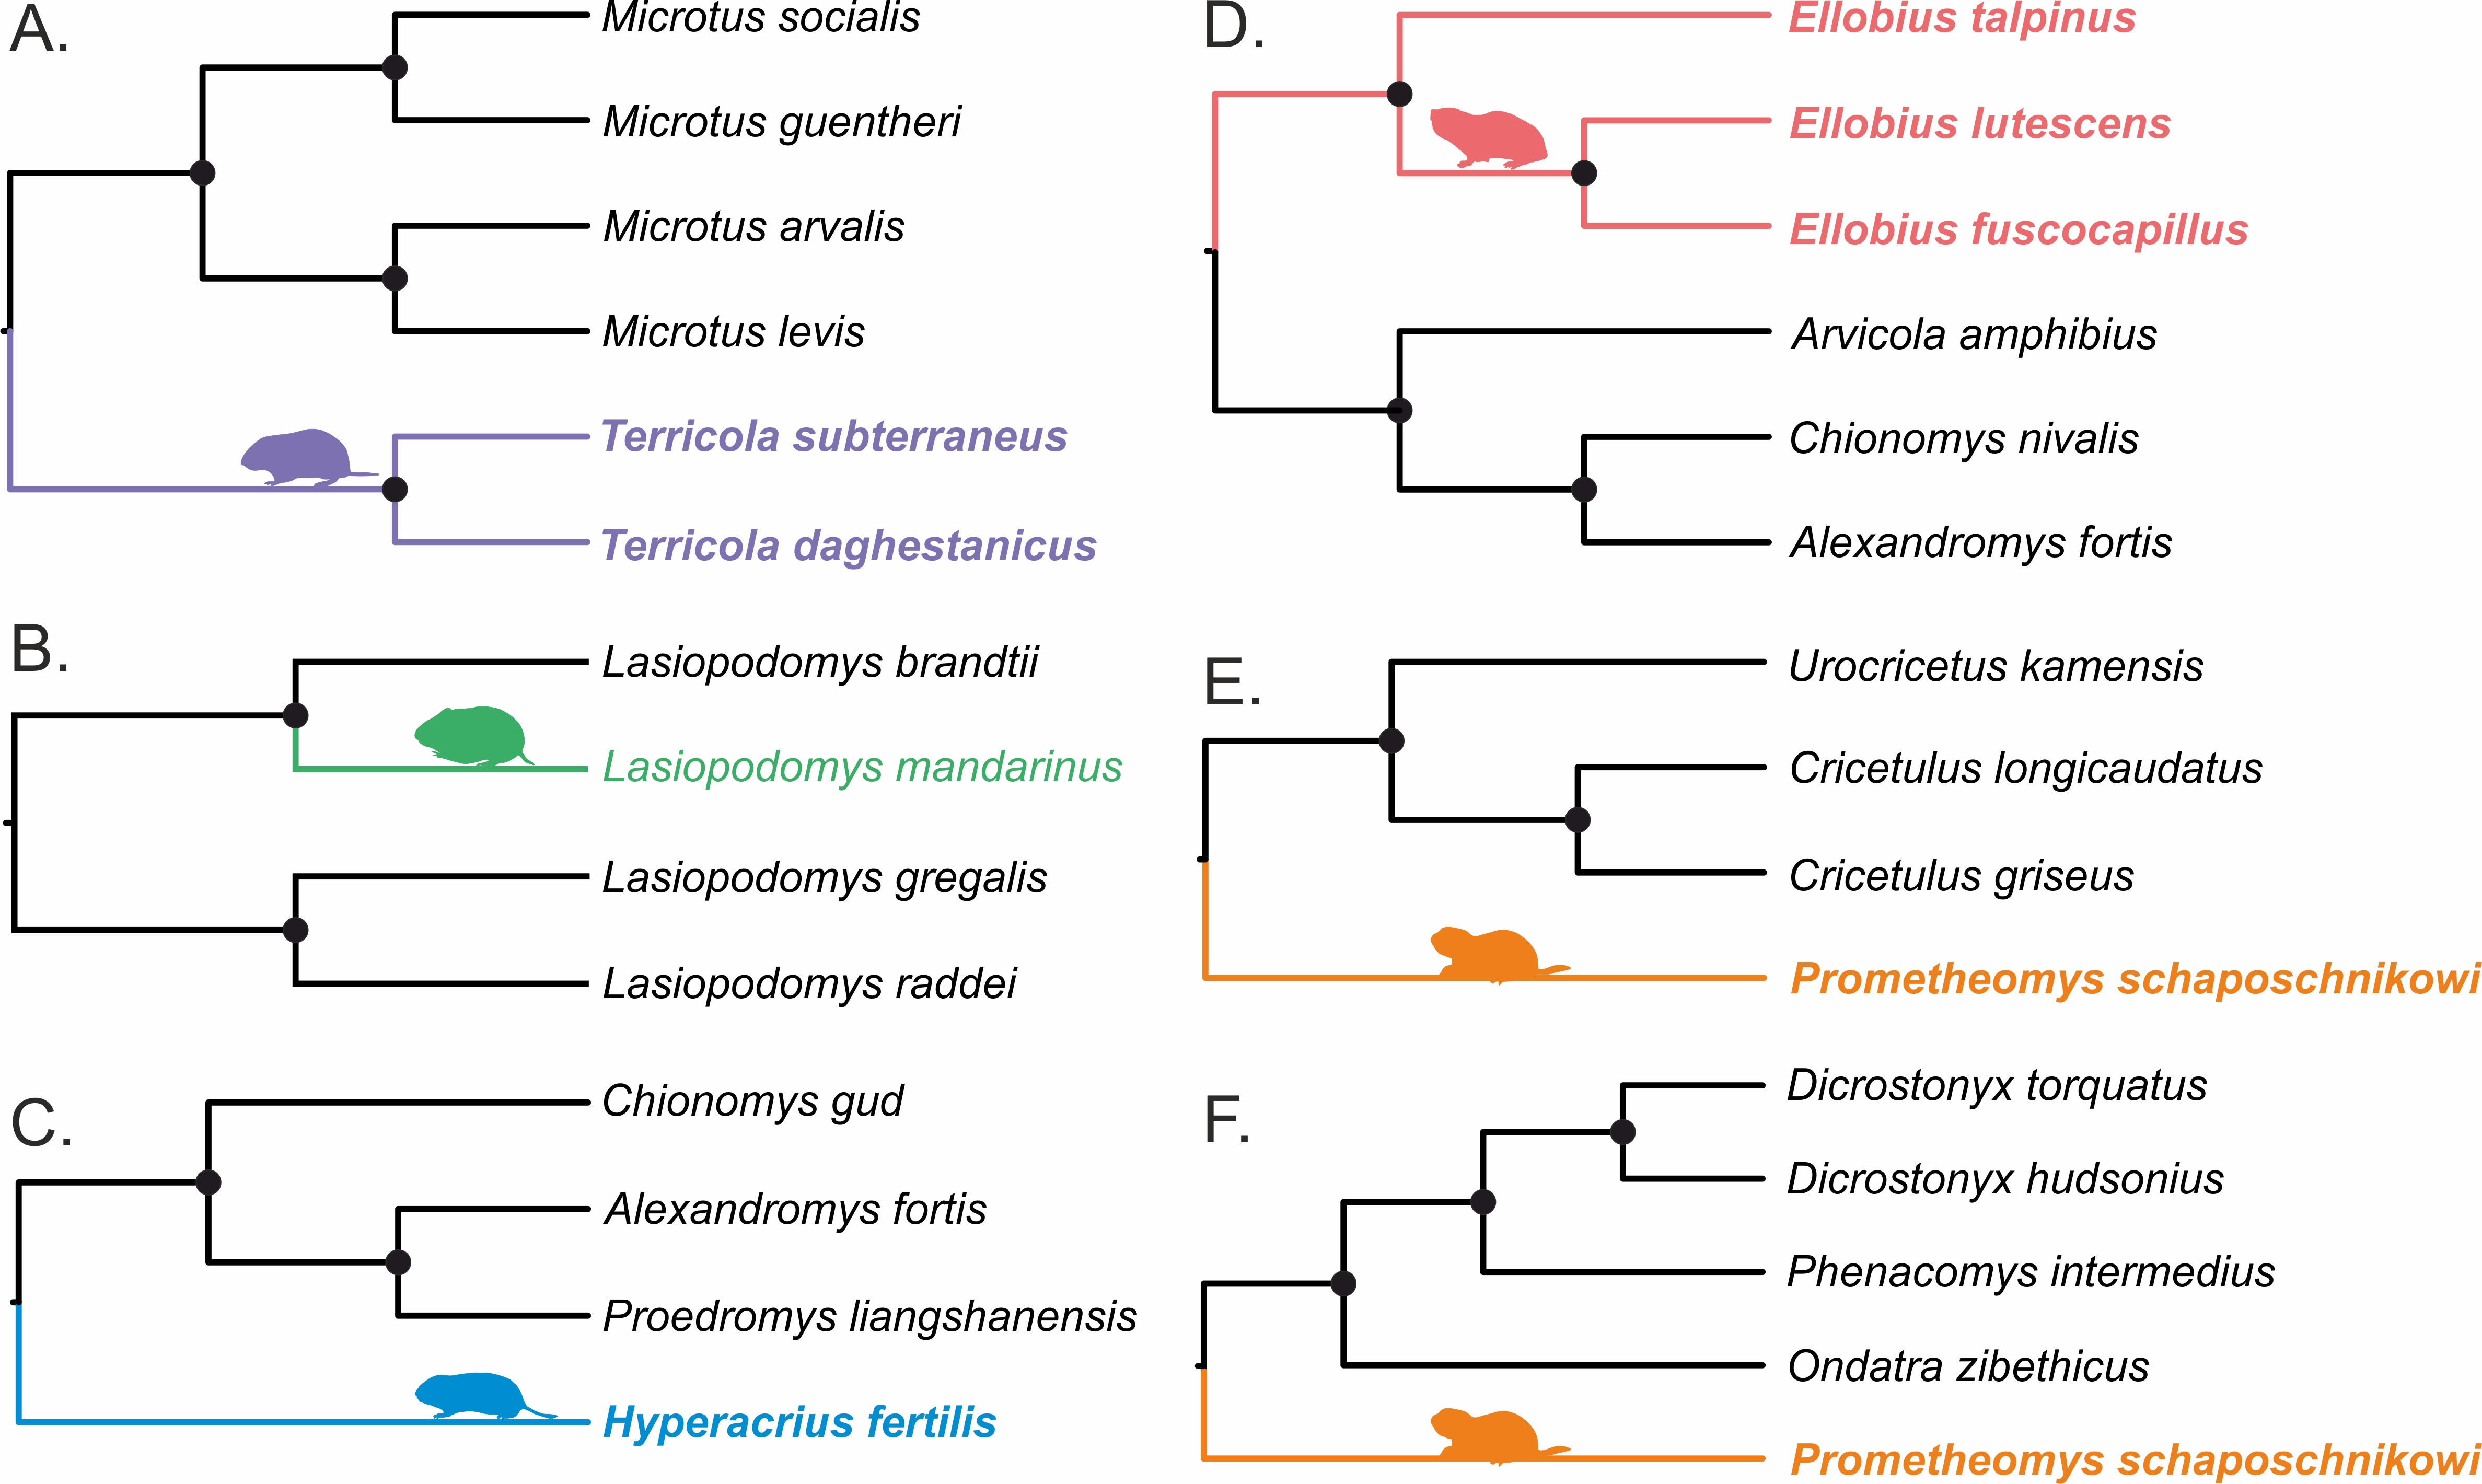
\includegraphics[width=\textwidth]{separate_mito_col}
	\end{center}
	\caption{Филогенетические деревья, использованные для оценки отбора по отдельным ветвям. Подземные виды обозначены цветом.}
	\label{tree_mito}
\end{figure}

\textbf{Моделирование и визуализация третичной структуры белка cytb}. Моделирование было основано на гомологии структуры \textit{Lemmus sibiricus} Kerr, 1792 и \textit{Ellobius lutescens} Thomas, 1897. За основу брали модель кристаллической структуры  \textit{Bos taurus} Linnaeus, 1758 с разрешением 2,4 Å (1NTM (\cite{Gao2003})). Программа modeller 9.22 (\cite{Webb2016}) использовалсь для создания структур комплекса протоколом автомоделирования с настройками по умолчанию. Замены были проанализированы визуально в PyMOL v.2.0 (Schrödinger, LLC). Трансмембранные участки комплекса оценивали с помощью веб-сервера OPM (\cite{Lomize2012}). 

\textbf{Предсказание сайтов фосфорилирования}. NetPhos 3.1 Server (http://www.cbs.dtu.dk/services/NetPhos/) (\cite{Blom2004}) и GPS 5.0 (http://gps.biocuckoo.cn/online.php) (\cite{Xue2011}) были использованы для предсказания изменения статуса фосфорелирования замен в гене \textit{CYTB}.


\subsection*{Глава 3. Характеристика собранных митохондриальных геномов и транскриптомов}

Всего в лаборатории эволюционной геномики и палеогеномики ЗИН РАН было собрано 34 новых митохондриальных генома представителей Arvicolinae. Анализ повреждений ДНК с помощью mapDamage для древнего образца \textit{Hyperacrius fertilis} показал низкое значение дезаминирования (рис. \ref{MapDamage}). Неправильное включение от C до T (красный) варьировалось от 12.09 \% до 17.94 \%, от G до A (синий) -- от 12.84 \% до 17.49 \%. Уровни ошибочного включения сравнимы со всеми другими вариантами замен, окрашенными в серый цвет, а также аналогичными значениям из статей (\cite{Molto2017}). Нами не было обнаружено каки-то структурных изменений в порядке генов или их количестве, которые отличали бы подземных грызунов от наземных сестринских видов. Результаты сравнения базовых нуклеотидных составов показали увеличение среднего значения \% GC и уменьшение GC-skew у подземных полевочьих, но разница в обоих случаях оказалась недостоверная.

\begin{figure}[h!]
	\begin{center}
		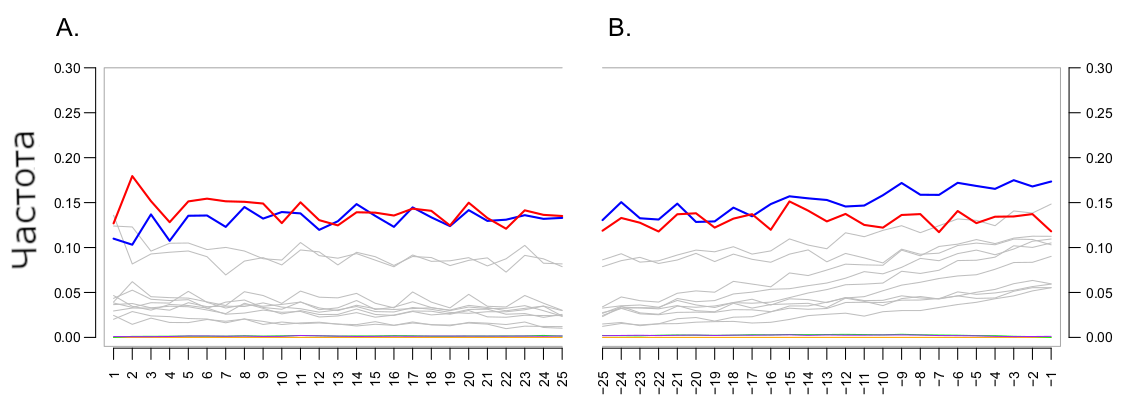
\includegraphics[width=0.8\textwidth]{MapDamage Hyper}
	\end{center}
	\caption{Дезаминирование нуклеотидов на 5` (А) и 3` конце (В), рассчитанные с использованием MapDamage. Все варианты замен отмечены серым, кроме замены гуанина на аденин (G>A, голубой цвет) и цитозина на тимин (C>T, красный цвет)}\label{MapDamage}
\end{figure}

В ходе работы нами было собрано 17 транскриптомов: сырые риды для 10 видов были полученных нами лично в рамках проекта РНФ и 7 взяты из открытой базы данных SRA, также мы использовали уже собранные транскриптомы для \textit{Microtus ochrogaster} Wagner, 1842 и \textit{Cricetulus griseus}. Статистика собранных транскриптомов показала, что все из них можно использовать в дальнейшем анализе. В них мы нашли 112 универсальных однокопийных ортологов. 
%После очистки собранных транскриптомов мы приступили к поиску универсальных однокопийных ортологов, которые присутствуют в одной копии у всех взятых в анализ видов. На этом этапе мы добавили к нашим данным два уже собранных и выложенных в базе данных Genome транскриптома: \textit{Microtus ochrogaster} Wagner, 1842 и \textit{Cricetulus griseus}. 


\subsection*{Глава 4. Оценка уровня и направления отбора}

\textbf{Ген \textit{CYTB}.} На первом этапе мы использовали 62 последовательности гена \textit{CYTB} представителей всех основных родов и триб Arvicolinae. Среди них были почти все филогенетически неродственные виды, перешедшие к существованию в подземной среде: представители рода \textit{Ellobius}, \textit{P. schaposchnikowi}, \textit{L. mandarinus}, \textit{T. subterraneus} и \textit{M. pinetorum}. Сравнение проводилось с наземными видами из 22 родов.  Оценка значений $\omega$ (отношение \textit{dN/dS}) у взятых в анализ видов показала общую тенденцию к ослаблению уровня отбора у подземных грызунов при сравнении их с филогенетически близкими наземными видами. Достоверные отличия в значениях $\omega$ получены с использованием программы codeml для видов рода \textit{Ellobius}, \textit{Lasiopodomys mandarinus} и \textit{Terricola subterraneus}. Почти у всех подземных видов наблюдаются более высокие значения $\omega$ по сравнению наземными, за исключением \textit{T. subterraneus}. Эта разница варьирует от одного (для \textit{Microtus pinetorum}) до пяти раз для \textit{Lasiopodomys mandarinus}. Тесты сравнения с нейтральной моделью (b\_neut) показали, что нуклеотидные последовательности гена \textit{CYTB} эволюционно не нейтральны у всех подземных грызунов. 

Анализ отбора алгоритмом aBSREL не показал свидетельств эпизодического отбора в анализируемой филогении. Результаты программы RELAX подтвердили изменения в уровне естественного отбора у подземных грызунов. Так, коэффициент отбора K для трех подземных представителей (\textit{Ellobius sp.}, \textit{L. mandarinus} и \textit{P. schaposchnikowi}) показал значения < 1, что может указывать на процесс ослабления отбора. 

Анализ распределения несинонимичных замен по сайтам показал три позиции с достоверно более высокими значениями частоты замен у подземных видов: 4, 237 и 241. Кроме того, в позиции 236 достоверно повышена частота синонимичных замен. Сравнение распределение замен по целым доменам (рис. \ref{Cyt_Dom_fig}) выявило значительные различия в мембранных доменах 1, 2, 5 и 9 и трансмембранных доменах 5 и 7 для несинонимичных замен; и мембранный домен 6 и трансмембранный домен 5 для синонимичных замен.

\begin{figure}[h!]
	\begin{center}
		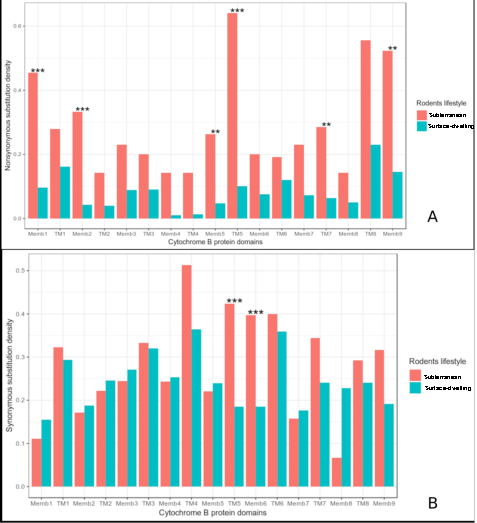
\includegraphics[width=0.7\textwidth]{cyt_domains}
	\end{center}
	\caption{Частоты распределения несинонимичных (A) и синонимичных (B) замен по доменам гена \textit{CYTB} у подземных и назменых грызунов. Достоверные различия между частотами обозначены звездочками(*): * -- p.value < 0.05, ** -- p.value < 0.01, *** -- p.value < 0.001 }\label{Cyt_Dom_fig}
\end{figure} 

\textbf{Митохондриальные белок-кодирующие гены.} 
%Для оценки количества замен в митохондриальных геномах использовали программу ProtParCon. Если подсчитать в целом количество несинонимичных замен, нормировав их на количество взятых в анализ видов, то наблюдается следующее: 
Доля несинонимичных замен в митохондриальных геномах подземных грызунов оказалось почти в два выше, чем у наземных. Отдельно в каждом гене эта тенденция повторяется.

При анализе программой codeml у представителей рода \textit{Ellobius} разница в уровне отбора наблюдается во всех митохондриальных генах, кроме \textit{ND2,3,5,6} и \textit{COX3} при сравнении с назмеными сестринскими видами. Несколько генов с достоверно отличающимся уровнем обнаружено также у \textit{L. mandarinus}: \textit{COX3} и \textit{CYTB}. Только один такой ген найден для \textit{P. schaposchnikowi} -- \textit{COX3}. У оставшихся представителей подземных грызунов не обнаружено генов с достоверным отличием от наземных видов. Значимые различия наблюдались в последовательностях \textit{COX3} и \textit{CYTB} для двух подземных видов одновременно: в \textit{COX3} для \textit{P. schaposchnikowi} и \textit{L. mandarinus} и в \textit{CYTB} для \textit{L. mandarinus} и представителей рода \textit{Ellobius}. Хотя значения $\omega$ существенно различались в зависимости от генов и анализируемых видов, значения $\omega$ не превышали единицы. Однако, все достоверно различающиеся значения $\omega$ были выше для подземных видов, чем для наземных. Используя алгоритм aBSREL мы обнаружили следы эпизодического положительного отбора в гене \textit{COX2} для \textit{E. lutescens} и в двух генах \textit{P. schaposchnikowi}: \textit{ATP8} при сравнении с видами Arvicolinae и \textit{ND5} при сравнении с хомяками. 

Анализ RELAX подтвердил изменения в уровне отбора подземных грызунов по сравнению с наземными. Семь генов для \textit{Ellobius} оказалось с K-значениями < 1: \textit{ATP6}, \textit{COX1}, \textit{COX3}, \textit{CYTB}, \textit{ND1}, \textit{ND2} и \textit{ND4} и столько же для \textit{P. schaposchnikowi} при сравнении с <<первой радиацией>> Arvicolinae: \textit{COX1}, \textit{COX3}, \textit{ND2}, \textit{ND4} и \textit{ND5}. Ген \textit{COX3} \textit{P. schaposchnikowi} также достоверно отличается от видов \textit{Cricetulus} по этому признаку. Список генов \textit{L. mandarinus} включает всего три: \textit{COX1}, \textit{COX3} и \textit{CYTB}. У оставшихся подземных грызунов: \textit{H.fertilis} и двух видов рода \textit{Terricola} гены с достоверным ослаблением или усилением отбора не обнаружены.

Многие гены выявлены у нескольких подземных полевочьих одновременно. Так, для генов \textit{COX3} и \textit{COX1} наблюдается ослабление отбора у видов рода \textit{Ellobius}, \textit{P. schaposchnikowi} и \textit{L. mandarinus}. Некоторые гены были обнаружены при анализе дважды для видов \textit{Ellobius} и \textit{P. schaposchnikowi} (например, \textit{ND2} и \textit{ND4}) или представителей \textit{Ellobius} и \textit{L. mandarinus} (\textit{CYTB}).

\textbf{Ядерные белок-кодирующие гены.} Сравнение частот несинонимичны замен между подземными и наземными видами не показало достоверных различий. Также нами не было обнаружено отдельных генов  или позиций, в которых частоты будут достоверно различаться. Мы провели поиск следов отбора в найденных нами ортологичных генах независимо для каждой линии подземных грызунов, однако, генов с достоверными отличиями обнаружено не было. 
 
\subsection*{Глава 5. Поиск параллельных аминокислотных замен и изучение их влияния на структуру белка}

%С помощью TreeSAAP мы получили список всех значимых аминокислотных замен (категории 6-8) для изучаемых видов в гене \textit{CYTB}. Из него мы выбрали те, которые встречаются по крайней мере у трех из подземных видов, но отсутствуют у всех наземных видов. 
Мы нашли три замены в гене \textit{CYTB}: Ser57Pro, Asp214Asn и Ile338Val (рис. \ref{PhyloTree}). Замена Asp214Asn была обнаружена также и у специализированных подземных грызунов из других семейств.

\begin{figure}[h!]
	\begin{center}
		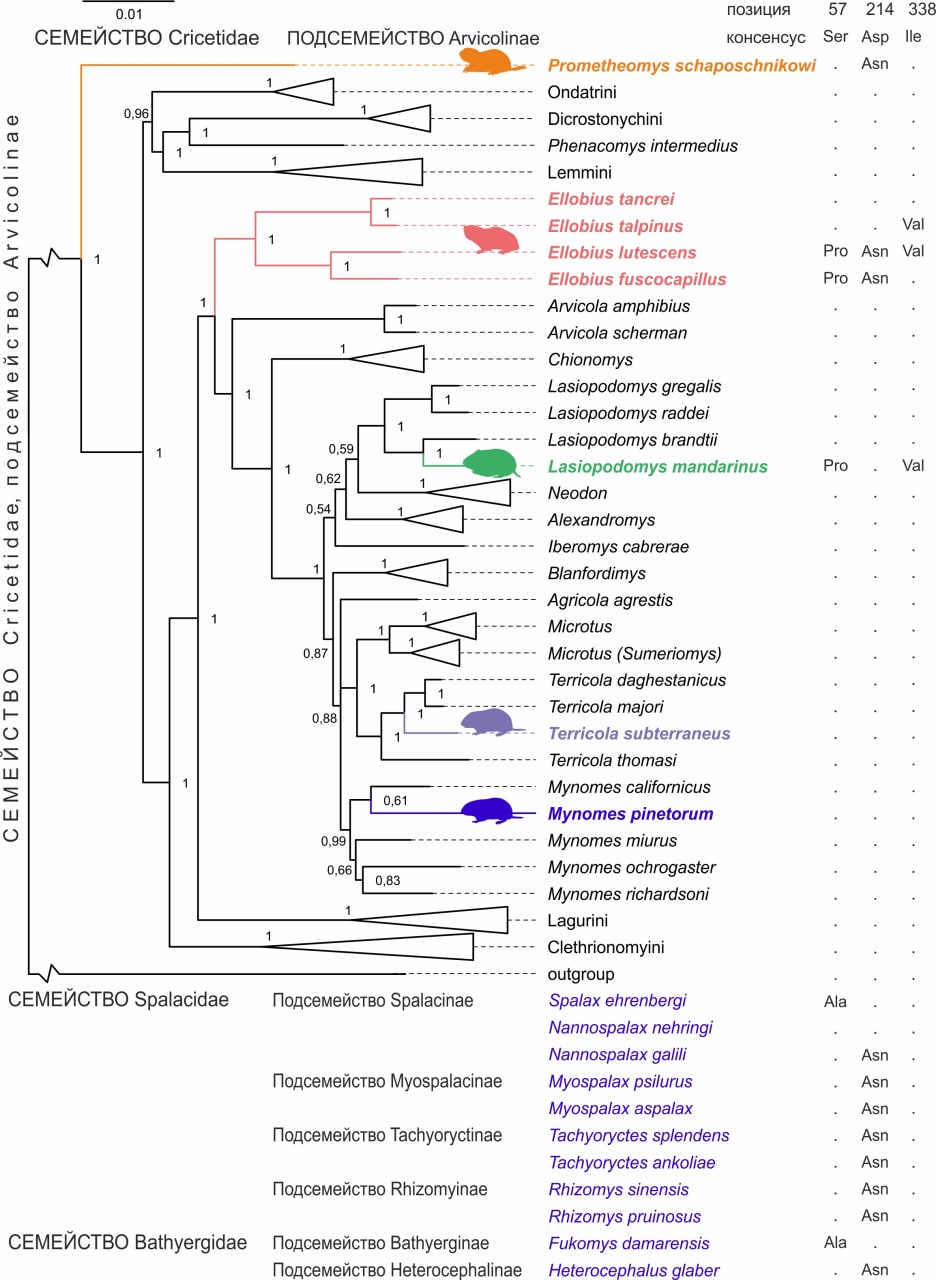
\includegraphics[width=0.9\textwidth]{Cytb_tree_colour_ed}
	\end{center}
	\caption{Филогенетическое дерево взятых в анализ видов. Указаны аминокислотные замены, характерные для подземных видов в гене \textit{CYTB}. Подземные виды отмечены цветом.}
	\label{PhyloTree}
\end{figure}

Замена серина на пролин в остатке 57 у подземных грызунов потенциально удаляет сайт фосфорилирования. Сервер NetPhos 3.1 предсказал фосфорилирование киназой \textit{CDC2} с оценкой 0,518. GPS 5.0 выявил киназы \textit{AGC}, \textit{PKN} и \textit{PKN1} с оценкой 65,363. Предсказания типа киназы не согласуются друг с другом, однако все прогнозы указывают на высокую вероятность фосфорилирования этого сайта. Те же методы не предсказывали фосфорилирование для Asp214Asn, и, насколько нам известно, ни Ile, ни Val в позиции 338 не могут быть фосфорилированы.

Нуклеотидная замена в кодоне 338 (ATT> GTT), приводящая к замене Ile338Val, был обнаружена как вероятный патоген в базе данных ClinVar и связана с раковыми процессами: www.ncbi.nlm.nih.gov/clinvar/variation/143898/.

Согласно третичной структуре белка цитохрома (рис. \ref{CytStructure} A), Ser57 обращен к межмембранному пространству митохондрий. Он расположен на неструктурированном сегменте петли, охватывающем остатки 54–60. Эта петля контактирует с той же петлей на втором мономере цитохрома \textit{bc1} в комплексе (рис. \ref{CytStructure} B). В отличие от Ser57Pro, замещение Asp214Asn находится на петле, обращенной к матрице митохондрии. Он контактирует с N-концом субъединицы VII комплекса убихинол-цитохром с редуктазы III (UQCRQ) (рис. \ref{CytStructure} C). Замена Ile338Val находится на границе раздела $\alpha$-спиралей в трансмембранной области комплекса (рис. \ref{CytStructure} D). Смоделированная структура показывает, что эта замена благоприятствует другому ротамеру Ile350, который соседствует с остатком 58 UQCRQ.

\begin{figure}[h!]
	\begin{center}
		\includegraphics[width=0.6\textwidth]{fig структура}
	\end{center}
	\caption{Структурная модель замен в комплексе цитохрома \textit{bc1}. \textbf{A.} Обзор гомодимера цитохрома \textit{bc1}. Цитохром Б --- голубой, UQCRQ - пурпурный. Второй мономер окрашен в желтый цвет. Места замены выделены кружками. IMS --- межмембранное пространство. \textbf{B.} Увеличенные структуры \textit{E. lutescens} и \textit{L. sibiricus}, показывающие замену Ser57Pro. Модель \textit{E. lutescens} голубая, \textit{L. sibiricus} --- белая. \textbf{C.} Замена Asp214Asn и его взаимодействие с N-концом UQCRQ (пурпурный) \textbf{D.} Замена Ile338Val и соседняя цепочка UQCRQ (пурпурный)}
	\label{CytStructure}
\end{figure}

При анализе белок-кодирующих митохондриальных генов были выявлены параллельные замены \textit{COX1} Met73Ile, \textit{COX3} Ile121Val, \textit{ND5} Phe446Leu, \textit{CYTB} Thr56Ser, \textit{CYTB} Ile338Val, \textit{CYTB} Ala357Thr. При дальнейшей статистической проверке все обнаруженные замены оказались недостоверными. 

Нами были обнаружены достоверные замены в ядерных генах \textit{Rad23b Thr121Ala} и \textit{Pycr2 Ala314Thr}.


\subsection*{Глава 6. Обсуждение результатов}

В нашей работе получены данные по изменению уровня отбора в митохондриальных генах подземных грызунов, а также обнаружены параллельные замены в ядерных генах. Помимо этого, мы сравнивали базовые характеристики митохондриальных геномов: GC-состав, его смещение, количество и порядок генов. 

\subsubsection*{Изменение нуклеотиного состава митохондриальных геномов}
Оценка GC-состава показывает повышение количества этих нуклеотидов у подземных грызунов. Уровень смещения (GC-skew) у подземных грызунов сильнее, чем у наземных грызунов. Несмотря на то, что разница в обоих случаях недостоверна, это может указывать на адаптивные следы в митохондриальном геноме. Генный состав митохондрий среди всех изученных видов остается стабильным и неизменным. Переход к подземному образу жизни не повлек за собой изменение в порядке генов или удвоению каких-то конкретных блоков.


\subsubsection*{Ослабление уровня отбора}
Исторически, изучение адаптивности митохондриальных генов началось с гена \textit{CYTB}. Начатые с трудов Эндрюс (\cite{Andrews1998}), и в последующем повторенные целым рядом исследователей (\cite{Tomasco2014}; \cite{DaSilva2009}; \cite{DiRocco2006}; \cite{Shao2015}), работы свидетельствовали о наличии признаков положительного отбора при эволюции гена \textit{CYTB}. Дальнейшие исследования показали, что, несмотря на сильные функциональные ограничения, митохондриальная ДНК в целом может подвергаться положительному направленному отбору, например, в случаях, когда требуется энергоемкий образ жизни и/или есть ограничения в доступности кислорода (\cite{Tomasco2011}; \cite{Shen2010}; \cite{Blier2001}).

Da Silva с коллегами (\cite{DaSilva2009}) обнаружили достоверную разницу в соотношении \textit{dN}/\textit{dS} ($\omega$) в независимых линиях подземных грызунов по сравнению с их наземными сестринскими видами. Это предполагает связь между эволюцией гена \textit{CYTB} и колонизация гипоксической среды. Позднее это наблюдение было подтверждено для всех митохондриальных белок-кодирующих генов \textit{Octodontidae} (\cite{Tomasco2011}).

В нашем исследовании гена \textit{CYTB} мы также обнаружили ослабление отбора у некоторых подземных грызунов. Применяя стандартные подходы, мы показали, что (1) несколько филогенетически далеких подземных видов имеют одинаковые аминокислотные замены в цитохроме b, и эти замены, вероятно, важны для структуры белкового комплекса, (2) в последовательности гена \textit{CYTB} повышено соотношение между несинонимичными и синонимичными заменами ($\omega$) у подземных грызунов по сравнению с наземными и (3) восемь белковых доменов обладают повышенной частотой замен у подземных видов, тоже наблюдается в нескольких нуклеотидных позициях. Эти результаты согласуются с гипотезой о том, что колонизация подземной ниши способствует положительному отбору в генах мтДНК.

Признаки усиления положительного отбора были выявлены как при сравнении четырех видов \textit{Ellobius} с \textit{Arvicola}, \textit{Eothenomys} и \textit{Chionomys}, так и у \textit{L. mandarinus} при сравнении с другими видами \textit{Lasiopodomys} и \textit{Neodon}. Мы обнаружили достоверную разницу в значениях $\omega$, анализируя \textit{T. subterraneus} с другими видами \textit{Terricola} и \textit{Microtus}, но в этом случае соотношение \textit{dN}/\textit{dS}, наоборот, было меньше для \textit{T. subterraneus}. Данные анализа RELAX согласуются с результатами codeml и показывают, что ген \textit{CYTB} у подземных грызунов подвержен ослаблению уровня отбора.


Результаты, полученные нами при исследовании всех белок-кодирующих митохондриальных генов, говорят о вовлеченности всего митохондриального генома в адаптивный процесс. Метод оценки отбора по отдельным ветвям (branch model codeml) показал повышение уровня отбора у подземных грызунов. Однако, мы наблюдаем различие в количестве генов с достоверным отличием у разных видов. Больше всего различий обнаружено у представителей рода \textit{Ellobius}: разница в отборе наблюдается во всех митохондриальных генах, кроме \textit{ND2,3,5,6} и \textit{COX3}. Два гена под отбором обнаружено у \textit{L. mandarinus}: \textit{COX3} и \textit{CYTB} и только один ген у \textit{Prometheomys} -- \textit{COX3}. У оставшихся представителей подземных грызунов не было обнаружено генов с достоверным отличием. Анализ RELAX подтвердил ослабление уровня отбора в митохондриальных генах у разных видов. Так, у представителей рода \textit{Ellobius} ослабление отбора наблюдается в 8 генах, у \textit{Prometheomys} --- в 5 (при сравнении с первой радиацией) и 1 при сравнении с хомяками. Для \textit{L. mandarinus} разница обнаружена в трех генах.  

Проводя поиск следов измнения отбора в генах подземных Arvicolinae мы обнаруживаем гены, которые показывают достоверные различия для более чем одного проанализированного подземного вида и гены, обнаруженные в более чем в одном анализе. Так, гены \textit{CYTB} и \textit{COX3} продемонстрировали более высокие значения $\omega$ одновременно у видов \textit{P. schaposchnikowi} и \textit{L. mandarinus} (\textit{COX3}) и \textit{L. mandarinus} и \textit{Ellobius} (\textit{CYTB}) при оценке уровня отбора методом codeml. Гены \textit{COX3}, \textit{COX1}, \textit{ND2} и \textit{ND4} демонстрируют ослабление отбора согласно программе RELAX по крайней мере для двух видов. Гены \textit{COX1} и \textit{COX3} были обнаружены как наиболее изменчивые при сравнении результатов нескольких программ. 


Набор генов с разницей в уровне отбора у подземных и наземных грызунов частично коррелирует со скоростью их эволюции. Скорости изменчивости среди семейств митохондриальных генов распределяются следующим образом: \textit{ATP}> \textit{ND}> \textit{CYTB}> \textit{COX} согласно Лопес (\cite{Lopez1997}). По нашим результатам, оба гена \textit{ATP} показывают достоверную разницу в уровне отбора для представителей рода \textit{Ellobius} по сравнению с назмеными видами. Кроме того, они выявляются в других анализах: RELAX (\textit{ATP6} для рода \textit{Ellobius}) и aBSREL (\textit{ATP8} для \textit{P. schaposchnikowi}). Гены семейства \textit{ND} показывают неоднородность в результатах. Среди всех генов этого семейства для генов \textit{ND2}, \textit{ND4} и \textit{ND5} обнаружены достоверные различия для трех из пяти проанализированных подземных видов. Ген \textit{CYTB} показывает достоверную разницу в уровне $\omega$ между подземными и наземными видами и подтверждает ослабление отбора для видов \textit{Ellobius} и \textit{L. mandarinus}. Эти результаты повторяют полученные при анализе отдельно гена \textit{CYTB} (\cite{Bondareva2021}). Неожиданный результат получен для генов семейства \textit{COX}: не смотря на свой консерватизм, они показывают достоверные изменения в уровне отбора во всех анализах на том же уровне, что и более вариабельные гены \textit{ND}.


Независимые исследования различных подземных грызунов показали адаптации в митохондриальных генах. Да Силва с коллегами (\cite{DaSilva2009}) обнаружили достоверную разницу в значениях $\omega$ в последовательностях \textit{CYTB} независимых линий подземных грызунов (\textit{Ctenomys},\textit{Spalacopus}, семейство \textit{Geomyidae} и семейство \textit{Bathyergidae}) по сравнению с их назмеными близкородственными видами (\cite{Tomasco2014}). Результаты Zhang предполагали, что эволюция гена \textit{CYTB} цокора \textit{Eospalax cansus} также в основном определяется изменением уровня отбора. Более того, распределение несинонимичных мутаций указывало на значительные изменения в последовательности \textit{CYTB} у животных, которые столкнулись с более тяжелой гипоксией из-за большей высоты и более холодного и сухого климата, чем другие митохондриальные линии (\cite{Zhang2013a}. Наконец, Tomasco и Lessa (\cite{Tomasco2011}) обнаружили повышенные значения $\omega$ в гене \textit{COX2} подземных восьмизубов (почти в 30X) и туко-туко (в 11X) по сравнению с наземными родственными видами. 


Позже указанные наблюдения были подтверждены для всех митохондриальных белок-кодирующих генов. Подземные виды южноамериканских туко-туко (\textit{Ctenomys}) и родственные восьмизубы (\textit{Spalacopus}) в работе Tomasco и Lessa (\cite{Tomasco2011}) показали достоверно более высокие значения $\omega$ по сравнению наземными видами в 11 из 13 митохондриальных генов. Конвергентные изменения были также обнаружены между изученными подземными видами и другими млекопитающими, адаптированными к гипоксии. Taveres и коллеги выявили достоверное ослабление отбора в большинстве митохондриальных генов подземных африканских землекопов, туко-туко и восьмизубов (\cite{Tavares2018}). 


С одной стороны, наши данные согласуются с опубликованным ранее работами и показывают, что митохондриальный геном подземных полевочьих потенциально вовлечен в процесс адаптации к подземному образу жизни. Но с другой, мы видим различие в уровне отбора между разными видами. Потенциально, это может быть связано с уровнем специализации к подземному образу жизни и его стилем.


К сожалению, обнаруженная на митохондриальных геномах тенденция к ослаблению отбора не подтвердилась на ядерных данных, и нам не удалось найти генов, уровень отбора в которых достоверно бы различался у подземных и наземных грызунов. Это может быть связано как с более медленными темпами эволюции (\cite{Lin2004}) по сравнению с митохондриальными генами, так и с недостаточным количествов генов, взятых в анализ. В работе Kalina Davies (\cite{Davies2018}), например, по исследованию адаптаций подземных млекопитающих только в 10\% от всех проанализированных генов (которых было около 8 тыс) обнаружена достоверная разница в отборе между подземными и наземными видами. 


\subsubsection*{Возникновение паралелльных аминокислотных замен}
Поиск параллельных замен показал себя как действенный способ обнаружить гены, которые могут быть вовлечены в адапционные процессы и при этом не меняют уровень или направление отбора (\cite{Davies2018}, \cite{Zhou2015}, \cite{Sackman2017}). 

При анализе отдельно гена \textit{CYTB} нами было обнаружено три замены, характерные для подземных грызунов: Ser57Pro, Asp214Asn, и Ile338Val. Замещение в сайте 57 также обнаружено у африканских слепышей (семейство Bathyergidae) и в 214 - у африканских слепышей и туко-туко (род Ctenomys). Аналогичное замены в сайте 214 были обнаружены у высокогорных подземных цокоров \textit{Eospalax fontanierii} (\cite{Cooper1993}). Cреди подземных полевок замена Asp214Asn была обнаружена у \textit{Prometheomys schaposchnikowi}, \textit{Ellobius fuscocapillus} и \textit{Ellobius lutescens}, а такая же у представителей большинства специализированных семейств подземных грызунов.

Выполняя изначальный поиск на одиночных генах (т.е. имея только один для одного вида), у нас была возможность проверить найденные замены на популяционном уровне в гене \textit{CYTB}. Использование его как основного филогенетического маркера позволило включить в полномасштабный популяционный анализ более 6 тыс сиквенсов. Из трех позиций, обнаруженных при анализе, две подтвердились: Thr56Ser и Ile338Val. В них мы видим достоверное смещение использования аминокислот у подземных грызунов: процесс ослабления отбора и большую вариативность в аминокислотном составе.

При анализе собранных митохондриальных геномах в митохондриальных генах нами было обнаружено шесть позиций с характерных для подземных грызунов заменами: \textit{COX1} Met73Ile, \textit{COX3} Ile121Val, \textit{ND5} Phe446Leu, \textit{CYTB} Thr56Ser, \textit{CYTB} Ile338Val, \textit{CYTB} Ala357Thr. Все выявленные замены оказались недостоверными при статистической проверке. 

Повторив поиск на ядерных геномах, нам удалось найти гены с параллельным аминокислотными заменами, которые есть только у подземных грызунов: \textit{Erp29}, \textit{Rad23b}, \textit{Hikeshi}, \textit{Zadh2}, \textit{Mrps14}, \textit{Pycr2}, \textit{Ccdc86}, \textit{GTPBP2}, \textit{Snapc2} и \textit{Ttll12}. Последующая проверка показала достоверность замен в генах \textit{Rad23b} и \textit{Pycr2}.

Согласно литературе, обнаруженное нами небольшое число генов (11\% от общего проанализированного числа) с уникальными заменами  является нормальным и ожидаемым. Так, в работе Kalina Davies (\cite{Davies2018}) было обнаружено всего 35 генов с паралельными заменами у всех проанализируемых видов (от общего количества проанализированных генов это меньше 1\%), а большее количество составляли гены с уникальными заменами (в нашей работе мы не рассматривали эти варианты) и парными среди разных родов. 

Найденные нами ядерные гены не выявлялись ранее при изучении подземных грызунов, в отличие от митохондриальных. Однако, биохимические пути и процессы, в которые они вовлечены, можно связать с процессами адаптации подземных грызунов. Активная работа митохондрий, которая может быть усилена в условиях сниженной концентрации кислорода, потенциально вызывает образование активных форм кислорода, являющихся опасным для клетки разрушающим фактором (\cite{Turrens2003}). Гены \textit{Rad23b} и \textit{Pycr2} (pyrroline-5-carboxylate reductase 2) связаны с процессами репарации ДНК (\cite{Pohjoismaki2012}) и реакцией на окислительный стресс (\cite{Kuo2015}), соответственно. Гомолог гена \textit{Rad23} был обнаружен при изучении адаптций к засухе у растений, поскольку его уровень отбора сильно изменялся в сторону положительного (\cite{Zhang2013b}). Изменение его экспрессии также выявлен при анализе устойчивости к холоду \textit{Thinopyrum intermedium} (\cite{Jaikumar2020}). 

\subsubsection*{Конвергентные адаптации грызунов к подземному образу жизни}
Мы наблюдаем у подземных полевочьих тенденцию проявления молекулярных адаптаций, описанную ранее в литературе, не смотря на ограниченную выборку полученных и проанализированных генов. В первую очередь, у них независимо ослабляется отбор на митохондриальных генах и увеличивается частота несинонимичных замен в целом. Как в митохондриальных, так и в ядерных геных происходят паралелльные аминокислотные замены в физиологически важных генах. 

По некоторым предположениям, повышение уровня отбора в митохондриальных генах могло быть следствем низкой эффективной численности популяции подземных грызунов (\cite{Lacey2000}). Однако, факты, что мы видим этот тренд 1) не во всех генах у одного рода и 2) не у всех видов подземных грызунов, скорее противоречит выдвинутой гипотезе. 

Анализ митохондриальных геномов и транскриптомов показал общие характеристики для подземных грызунов: увеличение уровня отбора и повышение частоты несинонимичных замен в митохондриальных генах, наличие параллельных аминокислотных замен как в митохондриальных, так и в ядерных генах. Однако, если анализировать каждую подземную линию независимо, видна неоднородность проявления этих признаков. Так, больше всего изменений затронуло род \textit{Ellobius}, а меньше всего -- \textit{Hyperacrius} (рис. \ref{common_trends_all}). Наблюдаемое количество изменений не коррелирует со временем дивергенции вида. Переход к подземному образу жизни у \textit{P.schaposchnikowi} произошел, согласно молекулярным данным, 7 млн лет назад. Но при этом вид не демонстрирует самое большое количество обнаруженных молекулярных изменений. В обоих случаях это наблюдается у представителей рода \textit{Ellobius}, хотя их переход к подземному образу жизни был совершен в плиоцене. Не смотря на это, морфологические изменения представителей этого рода наиболее близки к тем, что наблюдаются у <<модельных>> подземных грызунов семейств Bathyergidae и Spalacidae: выступающие резцы, очень маленькие глаза и изолирование ротового отдела губами (\cite{Gromov1977}). 

\begin{figure}[h!]
	\begin{center}
		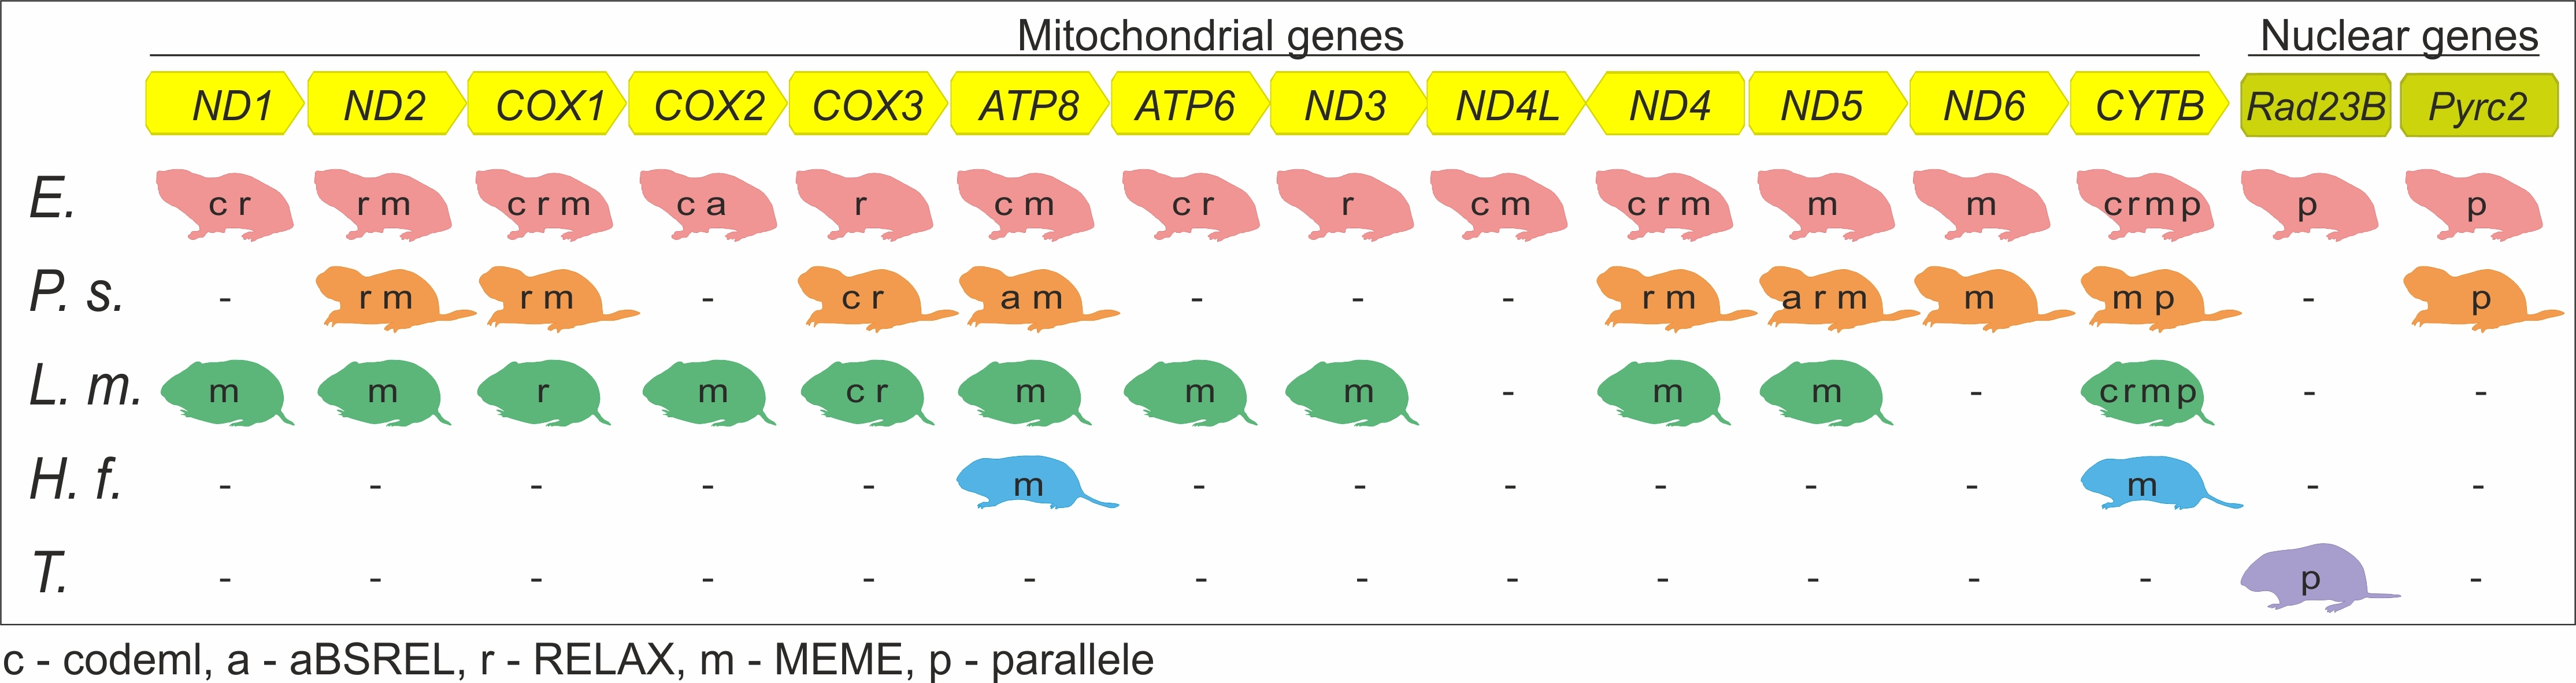
\includegraphics [width=0.9\textwidth]{genes_mt_and_nucl}
	\end{center}
	\caption{Общие тренды к изменению уровня отбора и возникновению параллельных замен у подземных грузынов подсемейства Arvicolinae}\label{common_trends_all}
\end{figure}

Самыми стрессовыми проблемами, с которыми сталкиваются подземные грызуны, являются гипоксические / гиперкапнические условия и перегрев в закрытой системе нор (\cite{Lacey2000}). Хотя и слепушонки, и \textit{P.schaposchnikowi} являются высокоспециализированными подземными грызунами, они занимают разные среды обитания, и характеристики их нор, а также методы добычи пищи весьма различны. Типичные места обитания \textit{Ellobius} --- засушливые или полузасушливые ландшафты, такие как степи, пустыни и луга. Эти грызуны населяют различные типы почв, в том числе плотные почвы глинистых пустынь, и создают довольно устойчивые системы узких туннелей для кормления под землей (\cite{Ognev1950}; \cite{Gromov1977}; \cite{Shubin1978}). Таким образом, слепушонки должны справляться с проблемами, с которыми сталкиваются другие действительно подземные млекопитающие (\cite{Lacey2000}). Последнее, в свою очередь, может привести к наблюдаемым нами изменениям в белок-кодирующих генах. Напротив, \textit{P.schaposchnikowi} встречается на кавказских субальпийских высокотравных лугах на высоте 1500-2500 м (\cite{Vereshchagin1959}; \cite{Vorontsov1966}; \cite{Krystufek2005}). Его норы вырыты в рыхлой влажной почве, заполненной камнями, что должно увеличить диффузию газа. Важно отметить, что поверхностные кормовые туннели этих полевок необычны тем, что они кажутся слишком большими и почти вдвое шире, чем можно было бы ожидать от грызунов такого размера (\cite{Vorontsov1966}; личные наблюдения АВС). Это дополнительное пространство может предотвратить перегрев, гипоксию и гиперкапнию. Кроме того, \textit{P.schaposchnikowi} строго травояден, по крайней мере, летом. Во время кормления полевка высовывается из норы, подбирает растения и затаскивает их в нору для безопасного кормления (\cite{Gambaryan1957}; \cite{Zimina1977}; личные наблюдения АВС). Таким образом, даже будучи ограниченными в поисках пищи вблизи отверстий для нор, они на самом деле проводят много времени вне туннелей. Благодаря холодному климату, архитектуре нор и особенностям кормления, \textit{P.schaposchnikowi} может избежать некоторых физиологических проблем, с которыми приходится сталкиваться большинству подземных видов.

У \textit{L. mandarinus}, не смотря на обнаруженные ранее изменения в циркадных ритмах и адатпации к гипокии (\cite{Sun2018}; \cite{Dong2020}), мы наблюдаем не такие сильные изменения в изученных нами генах: всего три гена с изменением уровеня отбора --- \textit{COX1}, \textit{COX3} и \textit{CYTB}. Тем не менее, мы обнаружили существенные различия у \textit{Lasiopodomys mandarinus} и \textit{Terricola}, несмотря на схожий эволюционный возраст этих таксонов. Это различие также может отражать неравные уровни энергетического и гипоксического стресса, возникающие из-за специфических характеристик стратегии поиска пищи и архитектуры норы. \textit{Lasiopodomys mandarinus} питаются либо под землей, либо зелеными частями растений в непосредственной близости от входа в нору. Кормовые ходы этого вида расположены на глубине 10-30 см (\cite{Smorkatcheva1990}; \cite{Hong2019}), а прямые измерения концентрации газов, температуры и влажности подтвердили, что животные в норе должны столкнуться с гипоксией и гиперкапнией. \textit{Terricola} населяют различные растительные сообщества от широколиственных лесов (\textit{T. subterraneus}) до альпийских лугов (\textit{T. daghestanicus}) (\cite{Aulagnier2018}). Подобно \textit{Ellobius}, \textit{Prometheomys} и \textit{L. mandarinus}, они используют сложную сеть подземных тоннелей и демонстрируют некоторые внешние черты, связанные с подземным образом жизни (например, \cite{Aulagnier2018}; \cite{Mironov2020}). Однако телосложение и повадки \textit{T. subterraneus} (Абрамсон и Сморкачева, неопубликовано), а также характеристики его туннельной системы отличают эту полевку от специализированных подземных грызунов. Пищевые пути этого вида располагаются в самом поверхностном слое почвы (в пределах 5-10 см) или даже непосредственно под опадой листьев (\cite{Mironov2020}). Туннели обеспечивают защиту полевок от неблагоприятных погодных условий и хищников, что объясняет тенденцию видов \textit{Terricola} к снижению скорости базовых метаболических процессов (\cite{Caroli2000}; \cite{Jemiolo1983}; \cite{Schropfer1977}), но их глубина, вероятно, слишком мала, чтобы существенно предотвратить диффузию газа, приводящую к гипоксическим / гиперкапническим условиям внутри. К сожалению, об экологии \textit{T. daghestanicus}, населяющего кавказские альпийские степи и луга, почти ничего не известно. Тот факт, что полевки этого вида, как сообщается, находят убежище среди скал (\cite{Krystufek2005}), предполагает, что они не так строго подземные. Наши результаты подтверждают этот факт, поэтому мы не обнаружили никаких изменений уровня отбора в митохондриальных генах этого вида. 

Подземные полевочьи повторяют адаптационный путь других подземных грызунов, показывая схожие признаки. Так, во время многочисленных исследований представителей семейств Bathyergidae и  Spalacidae были обнаружены паралельные замены в абсолютно разных генах. Также во многих генах видно ослабление отбора по сравнению с наземными. Этот эволюционный тренд подтверждается не только на подземных грызунах, но и на других подземных млекопитающих --  Talpidae и Chrysochloridae. Обнаруженные адаптации митохондриального генома (увеличение уровня отбора, наличие параллельных замен) совпадают с исследованиями на Octodontidae и Ctenomyidae. Таким образом, полученные нами результаты согласуются с гипотезой о том, что переход к подземному образу жизни стимулирует ослабление уровня отбора. Причем выраженность скорее связана с уровнем специализации вида, нежели с возрастом его появления.


\subsubsection*{Заключение}
В заключении кратко сформулированы основные результаты исследования.

\subsubsection*{Выводы}

\begin{enumerate}
	
	\item В гене \textit{CYTB} и митохондриальных генах обнаружено ослабление отбора у подземных полевочьих. 
	
	\item Параллельные замены у подземных форм полевочьих обнаружены в генах \textit{CYTB}, \textit{Rad23b} и \textit{Pyrc2}.
	
	\item Все гены с обнаруженными заменами вовлечены в процесс клеточного дыхания и репарацию.  
	
	\item Количество генов, в которых обнаружены ослабление отбора и параллельные замены, отличается у подземных полевочьих. Наибольшее количество генов с ослаблением отбора обнаружено у \textit{Ellobius}, \textit{Lasiopodomys} и \textit{Prometheomys}. Предположительно, это связано с уровнем специализации.
	
	\item Тенденции, выявленные у полевочьих в связи с переходом к подземному образу жизни на молекулярном уровне сходны с известными ранее у других древних специализированных подземных грызунов семейств Spalacidae, Ctenomyidae, Bathergidae.
	
\end{enumerate}


\newpage
\begin{small}
\subsection*{Список работ, опубликованных по теме диссертации}
\subsubsection*{В изданиях из перечня ВАК:}

\begin{enumerate}
\item[\textbullet] \textbf{Bondareva O. V.}, Abramson N. I. The complete mitochondrial genome of the common pine vole \textit{Terricola subterraneus} (Arvicolinae, Rodentia) //Mitochondrial DNA Part B. – 2019. – V. 4. – №. 2. – P. 3925-3926;
\item[\textbullet] Abramson N. I., Golenishchev, F. N., Bodrov, S. Y., \textbf{Bondareva, O. V.}, Genelt-Yanovskiy, E. A., \& Petrova, T. V. Phylogenetic relationships and taxonomic position of genus \textit{Hyperacrius} (Rodentia: Arvicolinae) from Kashmir based on evidences from analysis of mitochondrial genome and study of skull morphology //PeerJ. – 2020. – V. 8. – P. e10364;
\item[\textbullet] \textbf{Bondareva O. V.}, Mahmoudi, A., Bodrov, S. Y., Genelt-Yanovskiy, E. A., Petrova, T. V., \& Abramson, N. I. The complete mitochondrial genomes of three \textit{Ellobius} mole vole species (Rodentia: Arvicolinae) //Mitochondrial DNA Part B. – 2020. – V. 5. – №. 3. – P. 2485-2487; 
\item[\textbullet] \textbf{Bondareva O. V.}, Potapova, N. A., Konovalov, K. A., Petrova, T. V., \& Abramson, N. I. Searching for signatures of positive selection in cytochrome b gene associated with subterranean lifestyle in fast-evolving arvicolines (Arvicolinae, Cricetidae, Rodentia) //BMC Ecology and Evolution. – 2021. – V. 21. – №. 1. – P. 1-12;
\item[\textbullet] \textbf{Bondareva O.}, Bodrov S., Genelt-Yanovskiy E., Petrova T., Abramson N. Signatures of selection and adaptation to subterranean lifestyle across the transcriptomes of Arvicolinae (Rodentia, Cricetidae)// FEBS Open Bio. - 2021. - 11:P-01.3-17. doi:10.1002/2211-5463.13205;
\item[\textbullet] Abramson N. I., Bodrov, S. Y., \textbf{Bondareva, O. V.}, Genelt-Yanovskiy, E. A., \& Petrova, T. V.Mitochondrial genome phylogeny of voles and lemmings (Rodentia: Arvicolinae): evolutionary and taxonomic implications //Plos One. – 2021. - 16(11): e0248198;
\item[\textbullet]  \textbf{Bondareva O.}, Genelt-Yanovskiy, E., Petrova, T., Bodrov, S., Smorkatcheva, A., \& Abramson, N.  Signatures of Adaptation in Mitochondrial Genomes of Palearctic Subterranean Voles (Arvicolinae, Rodentia) //MDPI Genes. – 2021. – V. 12. – №. 12. – P. 1945.
\end{enumerate}

\subsubsection*{В сборниках конференций:}
\begin{enumerate}
	
\item[\textbullet] \textbf{Бондарева О.В.}, Петрова Т.В., Бодров С.Ю., Генельт-Яновский Е.А., Абрамсон Н.И. Следы отбора в митохондриальном геноме при адаптации к подземному образу жизни на примере представителей подсемейства полевочьих (Arvicolinae, Cricetidae, Rodentia) // материалы отчётной научной сессии ЗИН РАН по итогам работ 2019 г. (26--28 октября 2020, Санкт-Петербург). Издательство ЗИН РАН --- С. 11-13;

\item[\textbullet] \textbf{Olga Bondareva}, Semyon Bodrov, Natalia Abramson. Signatures of natural selection in mitochondrial genome of underground rodents. // Abstracts of the international conference on computer biology MCCMB`19 (July 27-30, 2019, Moscow) http://mccmb.belozersky.msu.ru/2019/index.html;

\item[\textbullet] \textbf{Bondareva O.}, Potapova N., Abramson N. Сan substitutions in mitochondrial protein sequence have adaptive signal? Сase study of voles and lemmings, subfamily Arvicolinae, Rodentia // VII International Congress and Associate Symposiums of Vavilov Society of Geneticists and Breeders on the 100th anniversary of the department of genetics of Saint Petersburg State University (June 18-22, 2019, Saint Petersburg, Russia). Book of abstracts. - P. 140.;

\item[\textbullet] \textbf{Olga V. Bondareva}, Artem Kasianov, Nataliya Abramson. Family-specified direction of selection in underground rodents // 6th International Conference of Rodent Biology and Management and 16th Rodens et Spatium (Potsdam, Germany, 3-7 September 2018), Book of Abstracts - P. 184 / 10.5073/jka.2018.459.000;

\item[\textbullet] Kristina V. Kuprina, \textbf{Olga V. Bondareva}, Antonina V. Smorkatcheva, Nataliya Abramson, Svetlana A. Galkina. Multiple mitochondrial pseudogenes in the nuclear genome in two species of mole voles (\textit{Ellobius}, Cricetidae) // 6th International Conference of Rodent Biology and Management and 16th Rodens et Spatium (Potsdam, Germany, 3-7 September 2018), Book of Abstracts - P. 148 / 10.5073/jka.2018.459.000/;

\item[\textbullet] \textbf{Bondareva O.}, Kasianov A., Abramson N. Do rodent species adopt to underground lifestyle by different ways? // The Eleventh International Conference (20–25 Aug. 2018, Novosibirsk, Russia); Abstracts. Institute of Cytology and Genetics, Siberian Branch of Russian Academy of Sciences; Novosibirsk State University. – Novosibirsk: ICG SB RAS, 2018. - P. 200 / DOI 10.18699/BGRSSB-2018-170;

\item[\textbullet] \textbf{Bondareva O.}, Chetverikova R., Rayko M., Abramson N. I. /Molecular adaptations of subterranean rodents to underground lifestyle. //  Abstracts of the international conference on computer biology MCCMB`17 (July 27-30, 2017, Moscow) http://mccmb.belozersky.msu.ru/2017/index.html.

\end{enumerate}


\end{small}
%%\bibliography{biblio}
